\documentclass{article}
\usepackage[margin=0.8in]{geometry}
\usepackage[utf8]{inputenc}
\usepackage{amsmath,amsthm,amssymb}
\usepackage{graphicx}
\usepackage{subcaption}
\usepackage{url}
\begin{document}
\title{Astronomy and astrophysics -- 1 \\
	   \large Assignment No.1 }
\author{Vishal Upendran, IUCAA}
\maketitle

This is the solution for the first assignment of the course Astronomy and Astrophysics -- 1 at IUCAA, Pune. The codes I used are available online\footnote{\url{https://github.com/Vishal-Upendran/Astro101/tree/master/Srianand_Assignment_1}}. 
\section{Question : 1}
We are given the coordinates of Proxima Centauri and the center of the triple system:
\begin{itemize}
\item Proxima Centauri ($\alpha$,$\delta$) = (14h26.3m,-62d29m)
\item Center ($\alpha$,$\delta$) = (14h36.2m,-60d36m)
\end{itemize}
Converting them to degrees, we get:
\begin{itemize}
\item Proxima ($\alpha$,$\delta$) = (216.575$^\circ$,-62.4833$^\circ$)
\item Center ($\alpha$,$\delta$) = ($219.05^\circ$,$-60.6^\circ$)
\end{itemize}
This gives us the angular separation between them as :
$$(\Delta\alpha,\Delta\delta) = (2.475^\circ,1.8833^\circ)$$
If we are to now assume the general position of an object on the celestial sphere in spherical coordinates, we have:
\begin{equation}
\begin{split}
&\bar{r} = \sin\delta\cos\alpha \hat{i} + \sin\delta\sin\alpha \hat{j}+\cos\delta \hat{k} \\
\Rightarrow &\cos\theta = \bar{r_1}.\bar{r_2} \\
\Rightarrow &\cos\theta = \sin\delta_1 \sin\delta_2 \cos(\alpha_1-\alpha_2)+\cos\delta_1\cos\delta_2
\end{split}
\end{equation}
Substituting our known values, and inverting $\cos$, we get:
$$\theta = 2.8879^\circ$$
Hence, we find the distance between the center and Proxima centauri from $l=R\theta$to be $l=2.016\times10^{17}$ cm.

For precessing the coordinates, we use:
\begin{equation}
\begin{split}
\Delta \alpha &= M+ N\sin\alpha \tan\delta \\
\Delta \delta &= N\cos\alpha \\
\end{split}
\end{equation}
M,N have a fitting equation as given in Caroll, Ostlie. Using this, we obtain: $$\Delta\alpha = 0.7672^\circ $$ $$\Delta \delta  = -0.1788^\circ$$ 

To obtain the change due to proper motion, first we have:
\begin{equation}
\mu = \frac{d\theta}{dt}=3.84''
\end{equation}
Where $\theta$ is the position angle, and $\mu$ the proper motion. Given this, we can formulate and solve for $\alpha$ and $\delta$ as:
\begin{equation}
\begin{split}
\frac{d\alpha}{dt} &= \mu\sin\theta\cos\delta \\
\frac{d\delta}{dt} &=\mu\cos\theta \\
\end{split}
\end{equation}
Solving, we obtain:
\begin{equation}
\begin{split}
\delta &= \mu\cos\theta t + c \\
\delta &=\delta_0 @ t=0 \\
\Rightarrow \delta &= \mu\cos\theta t + \delta_0 \\
\Rightarrow \alpha &=\mu\sin\theta\sin(\mu\cos\theta t + \delta_0)\frac{1}{\mu\cos\theta} + C
\end{split}
\end{equation}
Substituting for $\delta_0$, we get $$\Delta\delta = \mu\cos\theta t = 0.53^\circ $$
Hence, we can approximate $$\sin(\mu\cos\theta t + \delta_0) \approx \sin(\delta_0)$$ We thus obtain
$$\Delta\alpha = \mu\sin\theta\cos\delta t = -0.077^\circ$$

Thus we can see the change due to precession is much more than the change due to proper motion.
%----------------------------------
\section{Question : 2}
We are given the coordinates of the three objects. Converting them into degrees, we have:
\begin{center}
\begin{tabular}{|c|c|}
\hline 
$\alpha$ & $\delta$ \\
\hline 
329.89008 & 0.9138055 \\
329.496 & 0.95711 \\
329.3983 & 0.97127\\
\hline
\end{tabular}
\end{center}
With this information, we can download the appropriate files. 

The basic equation which holds for our objects of interest is:
\begin{equation}
\frac{f}{f_0} = 2b\sinh\left(-\left(\frac{m\times \log(10)}{2.5}+\log b\right)\right)
\end{equation}
Using the flux ratio $f/f_0$, we can obtain the flux in Jansky by:
$$f_\nu=3631*\frac{f}{f_0}$$
Since the SDSS fluxes are plotted per unit wavelength, we need to find an apt transformation. Thus, conserving energy, we have (ignoring the negative sign):
\begin{equation}
\begin{split}
d\lambda f_\lambda &= d\nu f_\nu \\
\nu = c/\lambda &\Rightarrow d\nu = -(c/\lambda^2)d\lambda \\
\Rightarrow f_\lambda &= \frac{c}{\lambda^2} f_\nu \\
\end{split}
\end{equation}
Now, we will need to convert such that one of the lambdas is in m (to cancel out the unit from $c$) and the other is in {\AA} for getting correct units. 
The plots for the different objects are shown in Fig.~\ref{fig:sdss}. 

It is interesting to see the fluxes don't match for the galaxies, and match well for the quasar. This might be due to the extended nature of the former two objects, causing a discrepancy in the measured flux. The quasar is not resolved, and is almost a point source, so the observed $f_\lambda$ agrees well with the computed $\lambda$.
\begin{figure}[!htpb]
\centering
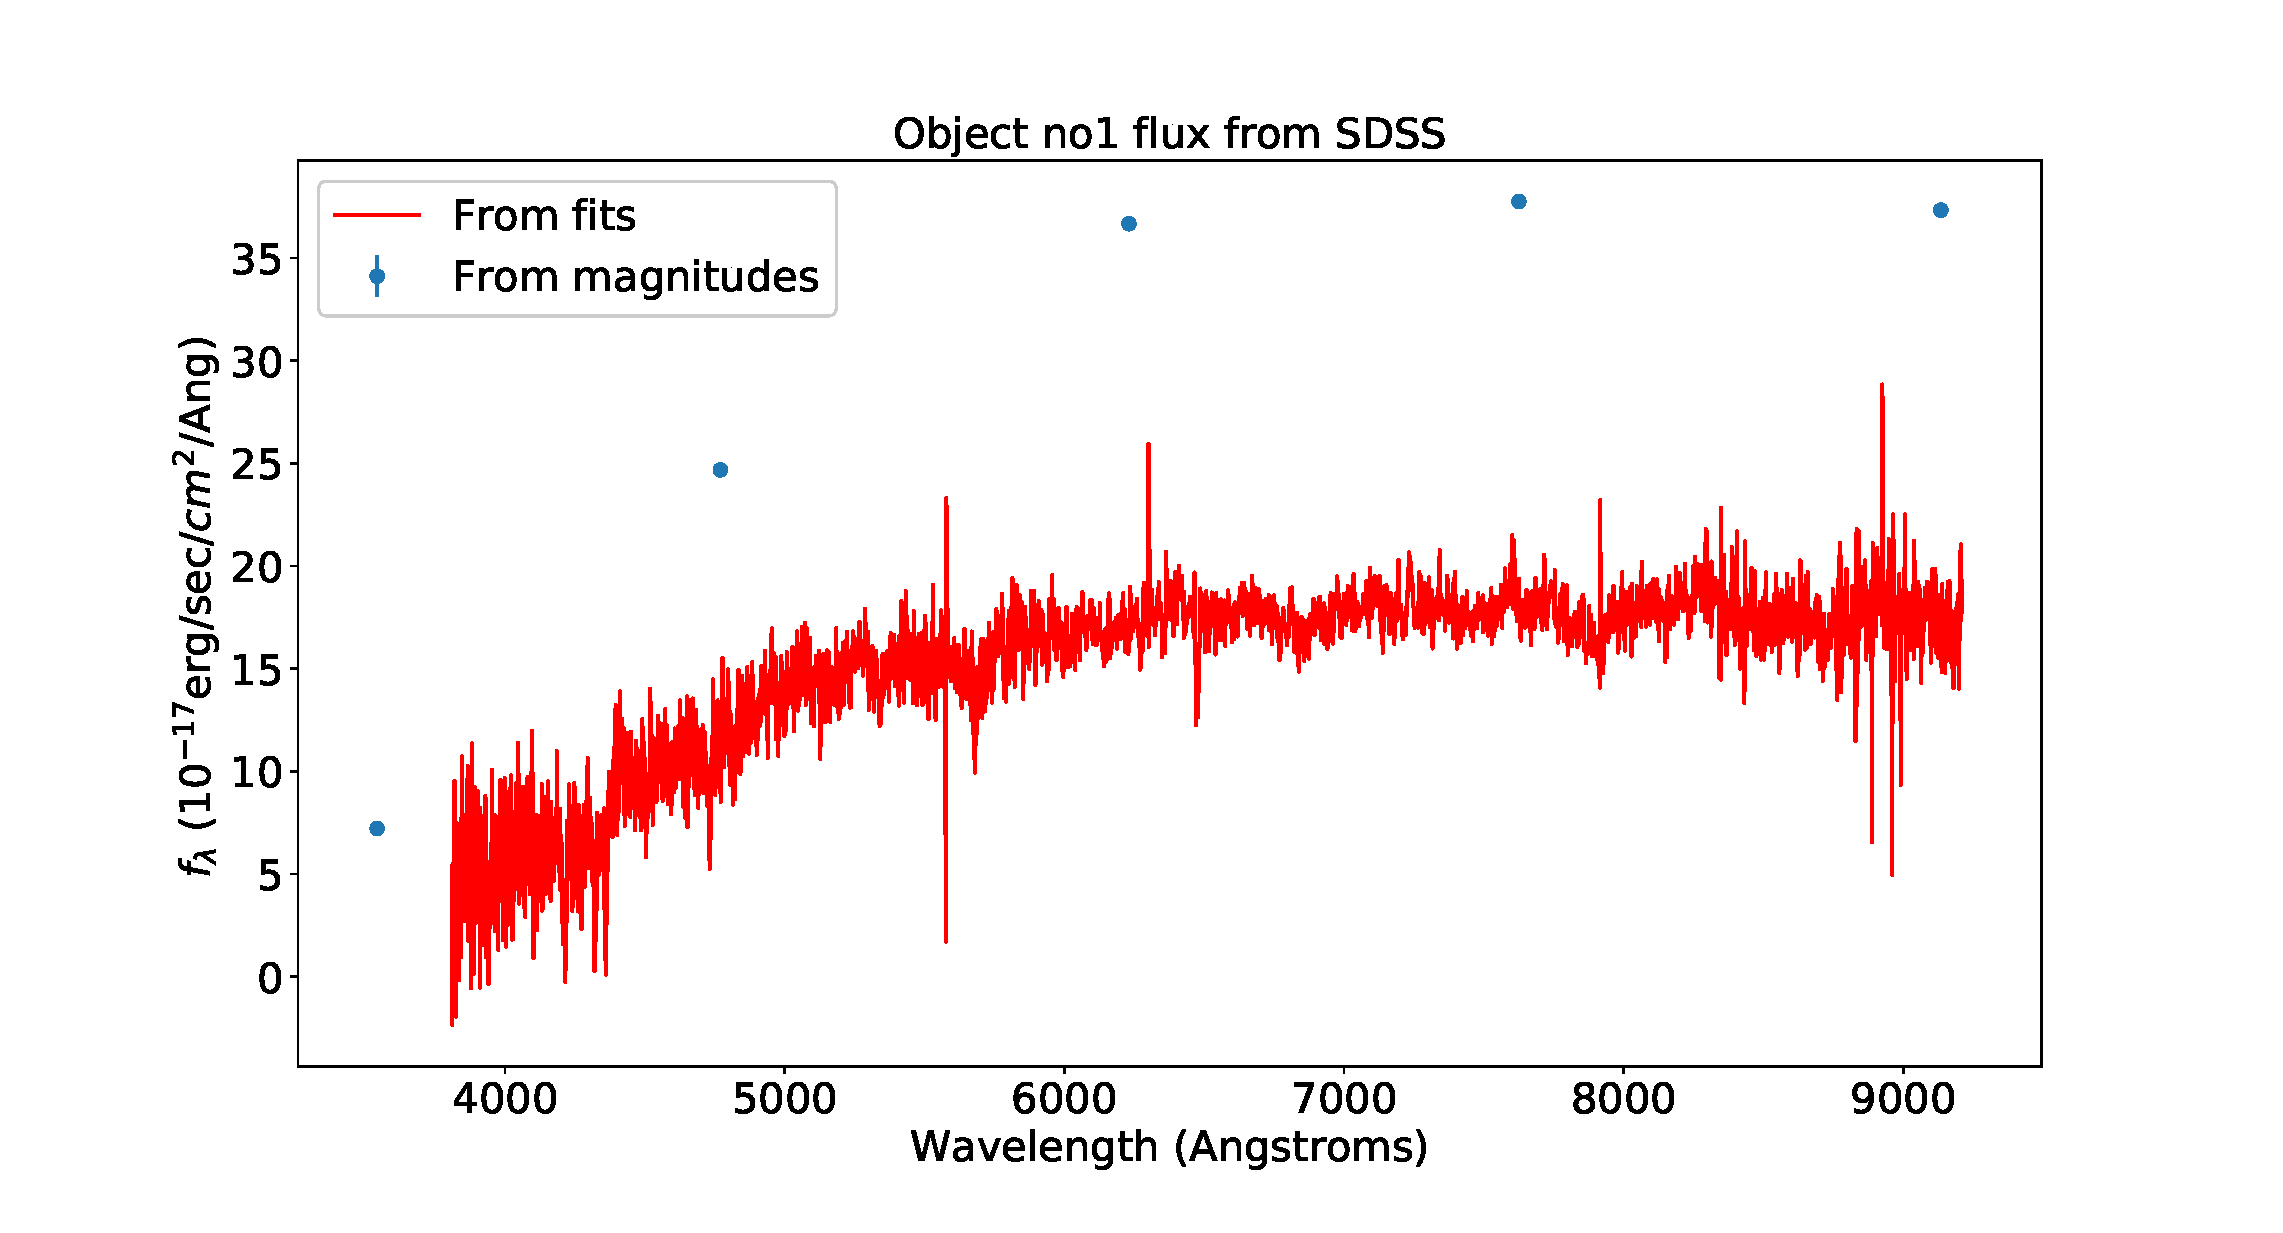
\includegraphics[width=0.8\linewidth]{Object_1.eps}
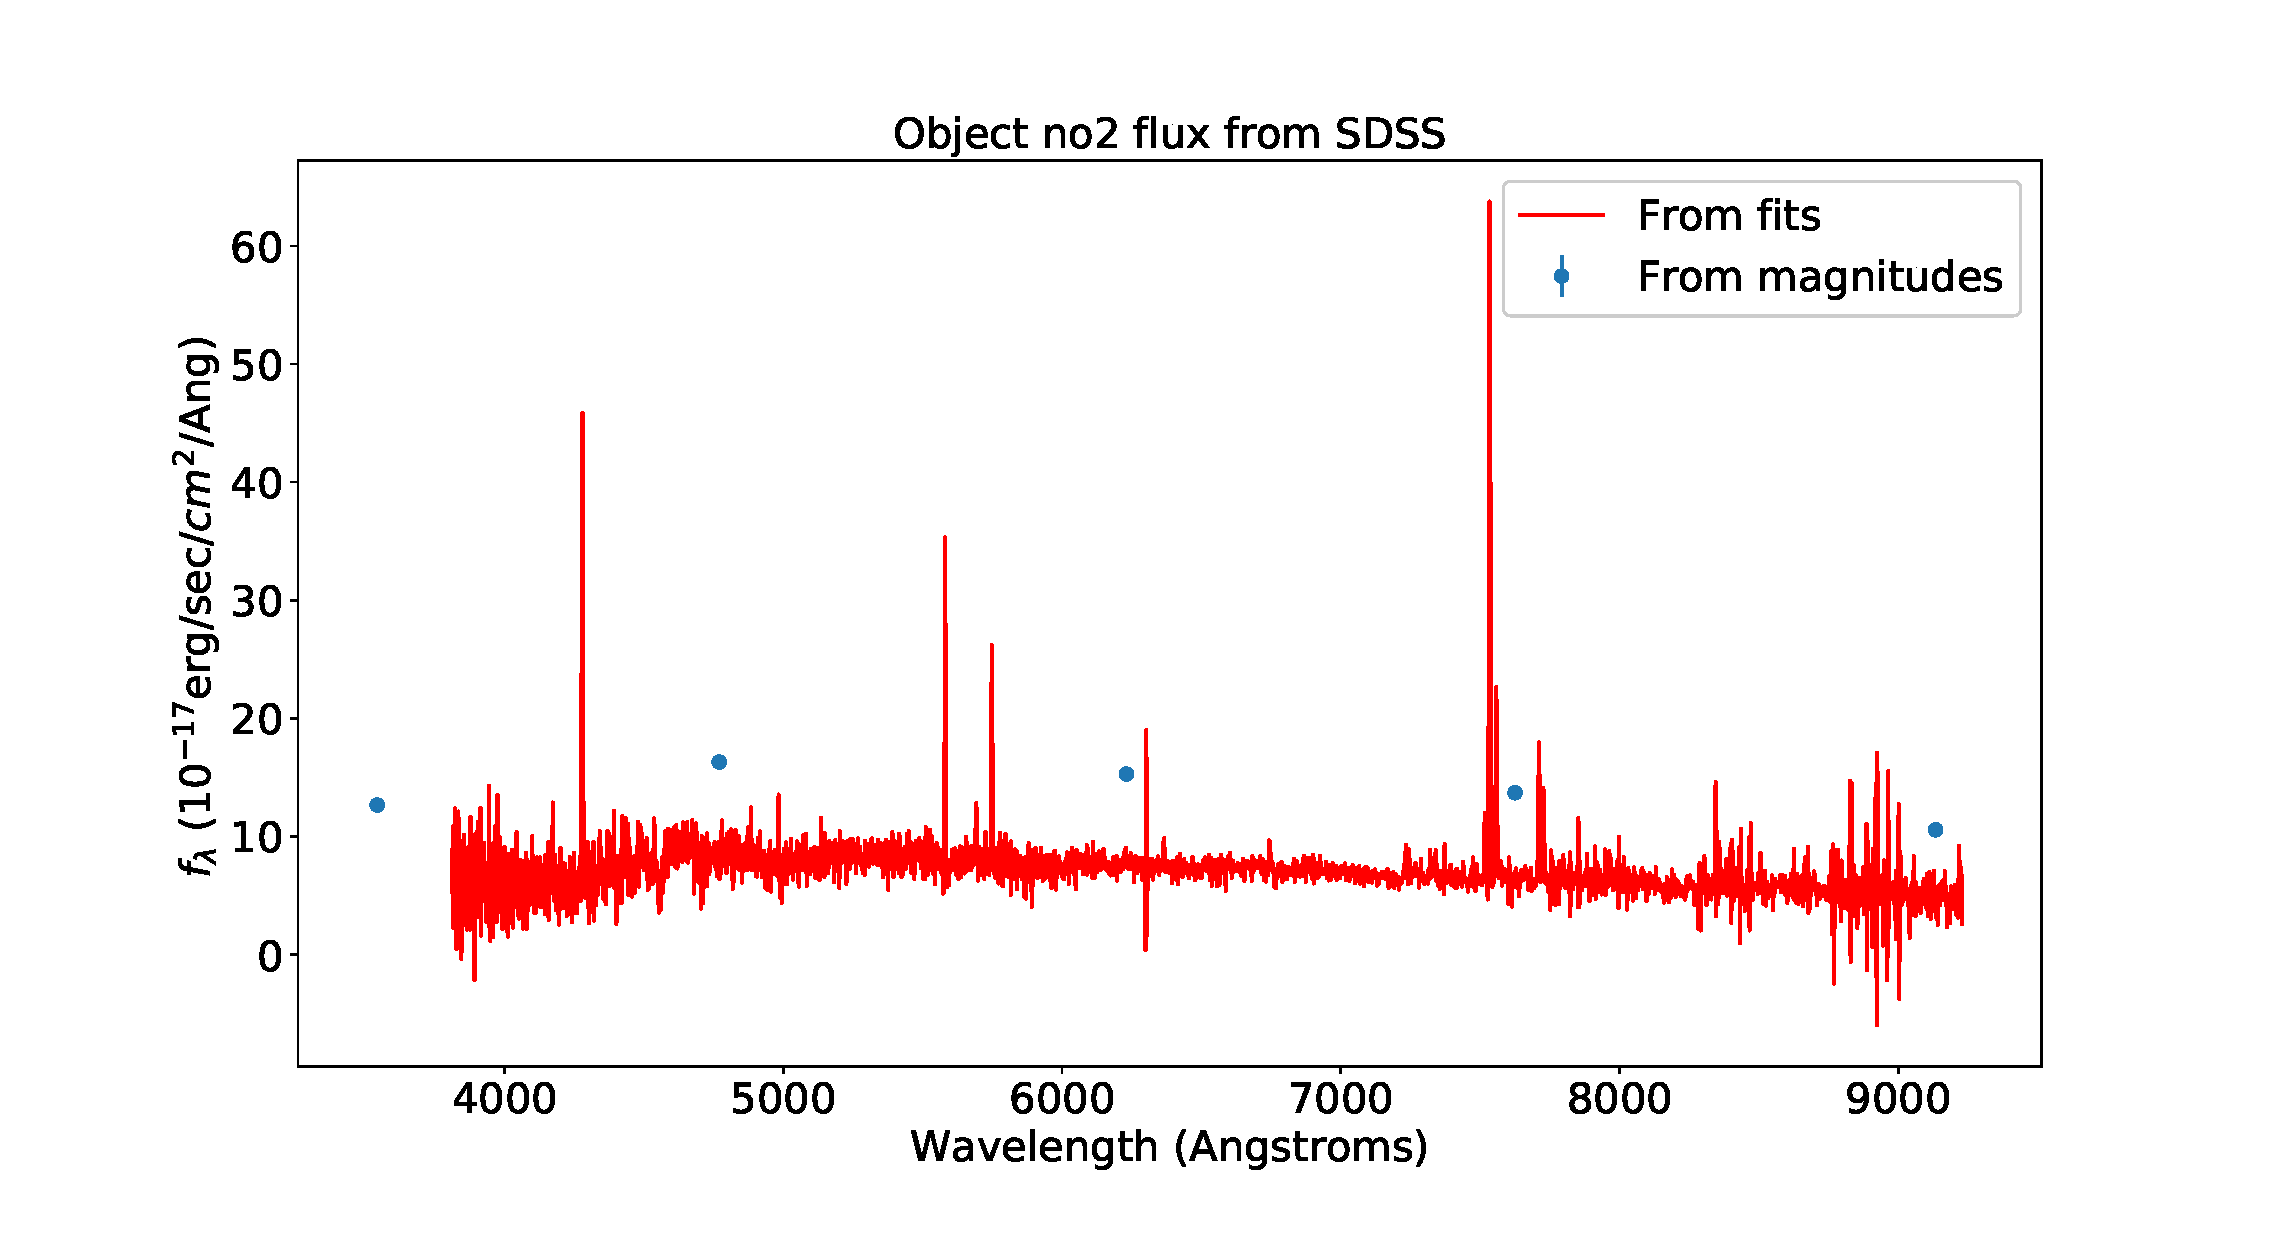
\includegraphics[width=0.8\linewidth]{Object_2.eps}
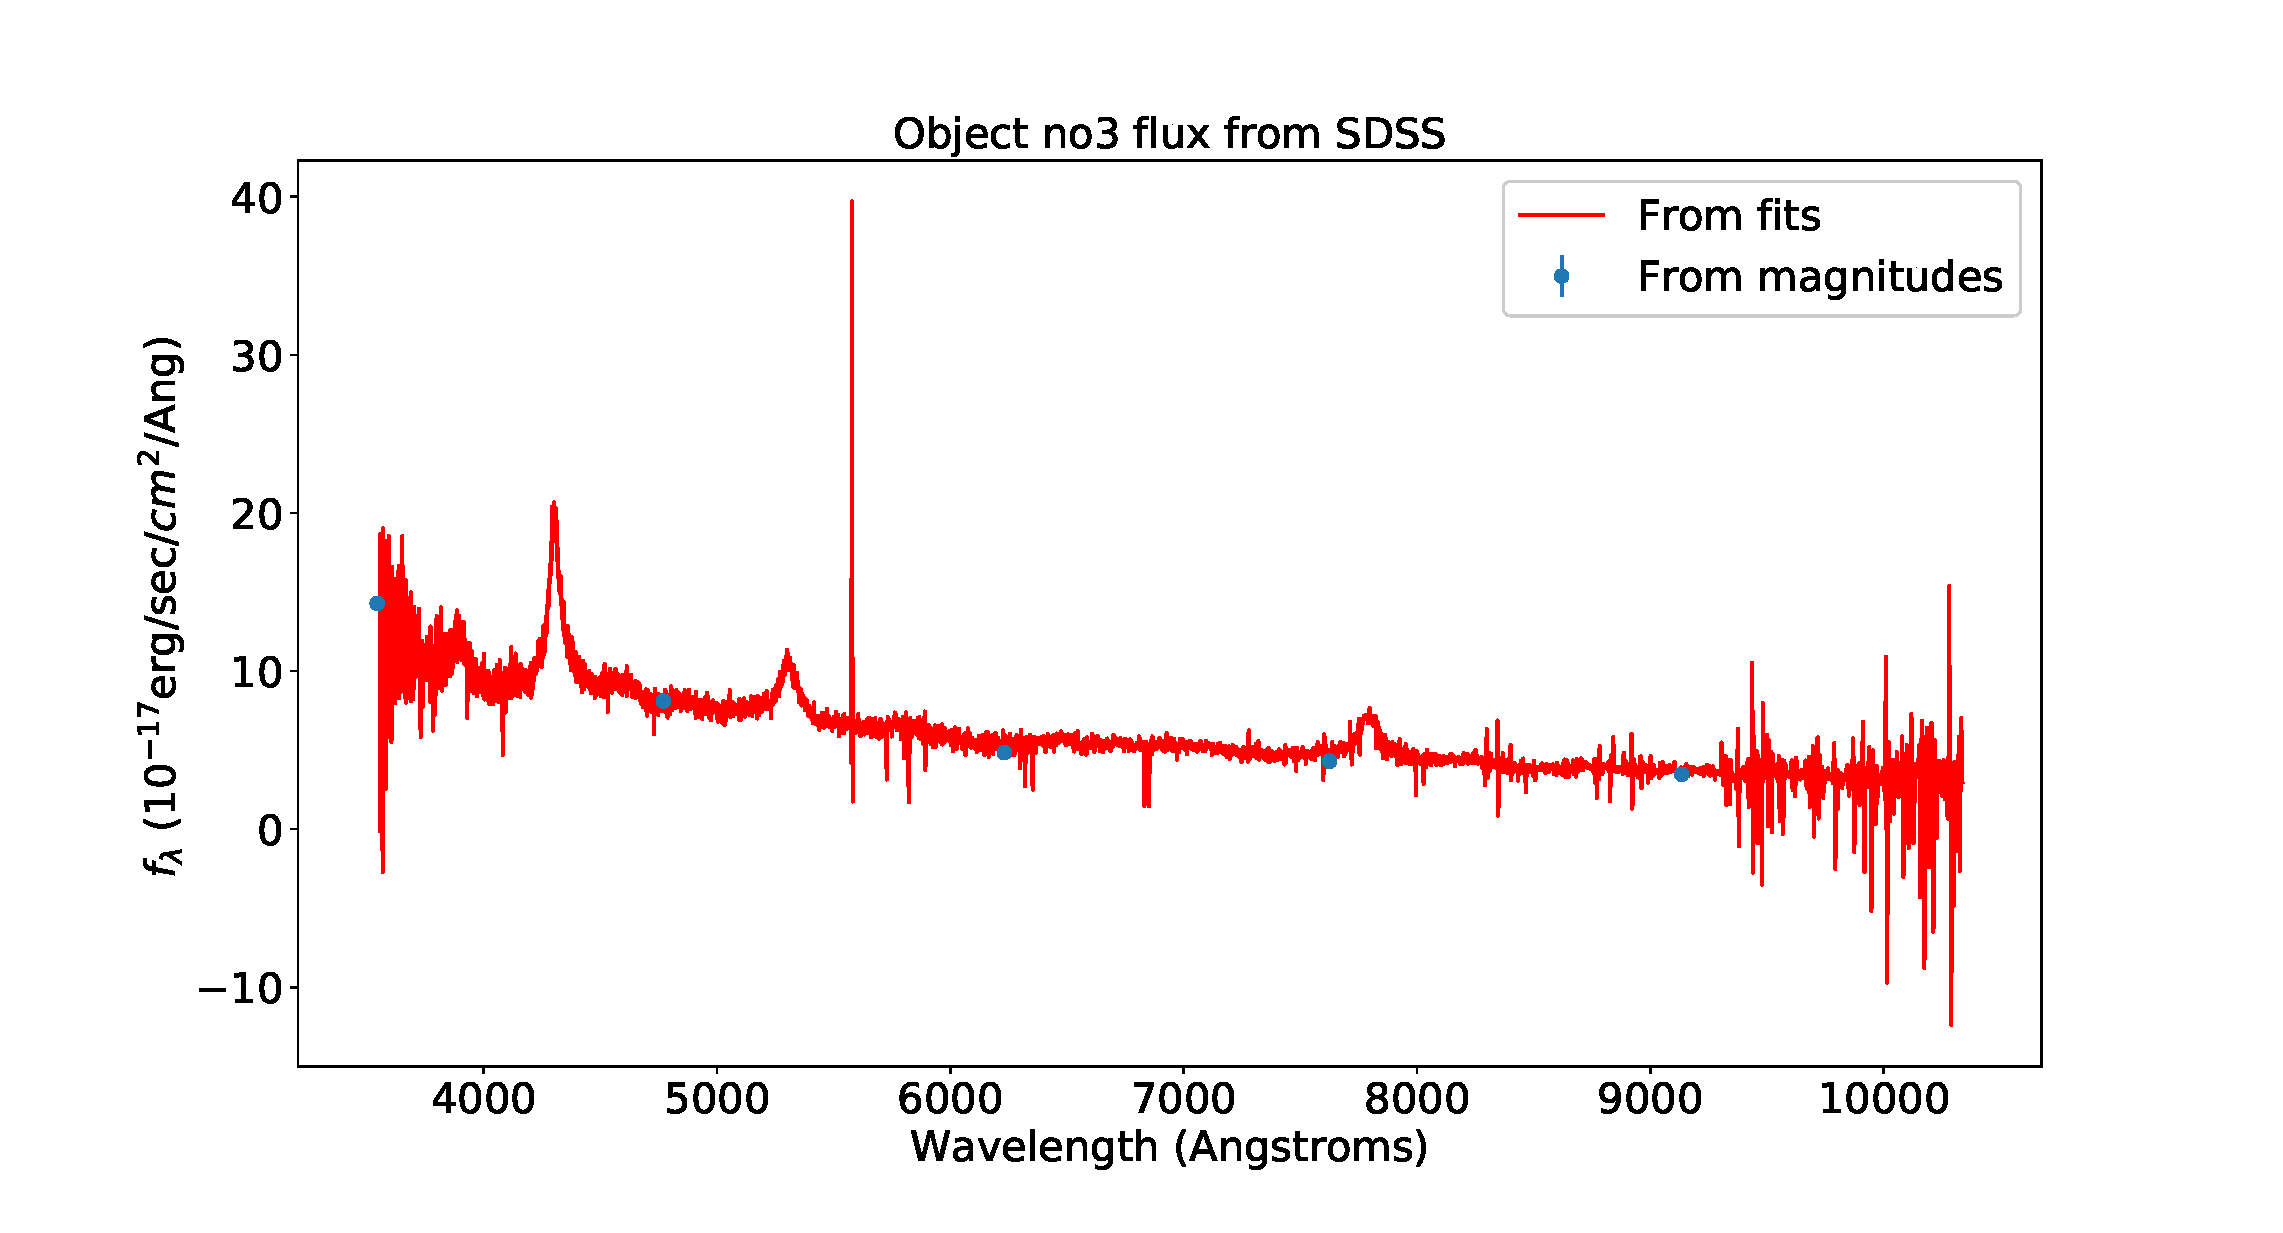
\includegraphics[width=0.8\linewidth]{Object_3.eps}
\caption{Calculated and observed flux per unit wavelength for Object 1 (top), Object 2 (middle) and Object 3 (bottom). The objects correspond to an elliptical galaxy, a star forming galaxy and a quasar respectively.}
\label{fig:sdss}
\end{figure}
%----------------------------------
\section{Question : 3}
We are given a very crude model of our galaxy, and asked to compute the no of stars visible for observation using an instrument of the given parallax angle. Thus, we also induce a number of approximations in our computation to make things easy.
First, we are given:
\begin{itemize}
\item Radius of galaxy: $10$ kpc
\item Height: $100$ pc
\item Total mass of galaxy: $10^{10}M_\odot$
\item All stars are like our Sun.
\item Trigonometric parallax: $0.005"$
\end{itemize}
For a parallax of $1"$, we get one parsec. Thus, for an angle of $0.005"$, we get:
$$
L_{max} = 200pc
$$
\begin{figure}[!h]
\begin{center}
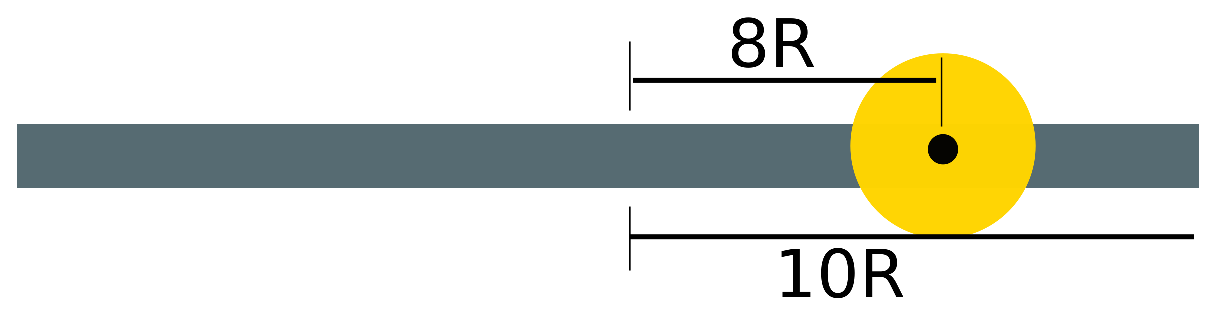
\includegraphics[width=\textwidth]{A_1_3.eps}
\caption{An illustration of how our field of view cuts the galactic disc. We need just consider the intersection of the two.}
\label{fig:3_1}
\end{center}
\end{figure}
Now, this angle holds if our object of interest lies along the normal of the equatorial plane, or on a plane perpendicular to the equatorial plane, this parallax angle traces out a circle. For any other orientation, it does not exactly trace out circles. However, we approximate the whole observable region to be a sphere. 
Next, we will need to find out the volume of the galactic disc scooped out by our sphere.  A visual aid is given in Fig.~\ref{fig:3_1}. Since our sphere radius is larger than the height of the galactic disc, we must consider only a small intersection of the two by removing the top and bottom parts of the sphere. Also, the profile inside traces out a spherical pattern, which is approximated to be a line due to the difference in height and the diameter of the sphere, essentially considering it to be a straight edge. Hence, we will need to find the volume of the sphere of height $100$ pc, and radius of intersection. Using Pythagoras, we have:
\begin{equation}
\begin{split}
r_{cyl} &= \sqrt{200^2-50^2} \\
&\approx 193.6
\end{split}
\end{equation}
Where all the numbers are in parsec. . Furthermore, we know the approximate distance of our solar system from the center of the galaxy as shown in Fig.~\ref{fig:3_1}. This results in our distance from center $\approx 800$ pc, which is much greater than our radius. Thus, for the no. of stars visible, we have:
\begin{equation}
\begin{split}
N & = 10^{10}\times\frac{\pi 193.6^2 100}{\pi 10^8 100} \\
&=10^{10}\frac{37500}{10^8} \\
&=3.75\times10^{6} \\
&\approx 10^6
\end{split}
\end{equation}
Hence, we can observe a million stars using our instrument.
%-------------------------------------
\section{Question : 4}
{
This question asks an estimate on the number of stars present in a galaxy, with the following information given:
\begin{itemize}
\item Apparent magnitude of galaxy $m_{g}$ = 30
\item Distance to galaxy $d_{g}$ = 3$\times$ $10^9$ pc
\item Luminosity of the galaxy $L_{g}$ = N $\times L_\odot$
\item Absolute magnitude of Sun $M_\odot$ = 5
\end{itemize}
The idea is to first find out the apparent magnitude of the Sun, and then compare the apparent magnitudes of the galaxy and Sun. The comparison is made simple for the stars in the galaxy are assumed to have the same intrinsic luminosity as Sun. Thus, for our Sun we get:
\begin{equation}
m_\odot - M_\odot = 5 log_{10} \frac{d}{10} 
\end{equation}
where $d$ is measured in parsecs, which would be 1 A.U in parsec. However, let us simply the equations before plugging in the numerics. Simplifying, we get 
\begin{equation}
m_\odot = M_\odot + 5 log_{10} \frac{d}{10} 
\label{eq4:1}
\end{equation}
Now, comparing the two apparent luminosities, we get:
\begin{equation}
m_g - m_\odot = -2.5 log_{10} \frac{L_{g} 4 \pi d^2}{L_\odot 4\pi d_g^2}
\label{eq4:2}
\end{equation}
Simplifying, and substituting Eq.~\ref{eq4:1} in Eq.~\ref{eq4:2}, we get:
\begin{equation}
\begin{split}
m_g &= m_\odot - 2.5 log_{10}\frac{NL_\odot d^2}{L_\odot d_g^2} \\
m_g &= M_\odot + 5log_{10}\frac{d}{10} - 5log_{10}\frac{d}{d_g} - 2.5log_{10} N \\
m_g & = M_\odot -5log_{10}\frac{10}{d_g}-2.5log_{10} N \\
25 &= -2.5log_{10} N\frac{100}{d_g^2} \\
\Rightarrow N &=10^{-10}.9.10^{16} \\
\Rightarrow N &=9\times10^6
\end{split}
\end{equation}
Thus, the galaxy contains approximately a million stars. 
}
\section{Question : 5}
We are asked to find how far a star is away from us, given:
\begin{itemize}
\item It has a planet going around with a period of 80 years. 
\item The separation of star and the planet is 20 arcsec.
\item The star is Sun-like. So we use $M_s$ = $M_\odot$
\end{itemize}
We assume the orbit is circular, and is face-on, thus the separation between the sun and the planet is almost always 20arsec. Now, by Kepler's third law, we have:
\begin{equation}
T^2 = \frac{4\pi^2}{GM} r^3
\label{eq5:1}
\end{equation}
Using the standard values for the constants, and solar mass, we get 
\begin{center}
$R = 2.7\times 10^{12} $ m
\end{center}
Thus, using parallax, we get:
\begin{equation}
\begin{split}
R &= D\theta \\
\Rightarrow D &= 2.78 \times 10^{16} m = 0.9 pc
\end{split}
\end{equation}
%----------------------------------
\section{Question : 6}
Hydrostatic equilibrium is not possible for an isothermal constant density gas, for if that were the case there would not be any gradients to support gravity, i.e:
\begin{equation}
\frac{dP}{dr} = -\frac{GM\rho(r)}{r^2} 
\label{eqn6:1}
\end{equation}
$$P \propto \rho \equiv Const $$
Thus, the pressure gradient would be zero on the L.H.S of Eq.~\ref{eqn6:1}, thus not supporting gravity. 

We are next given a density profile and asked to calculate the pressure profile. The density is given by:
\begin{equation}
\rho(r) = \frac{\rho_c}{1+(r/r_c)^2}
\end{equation}
We first find the mass contained in a sphere of radius r, and this is obtained as:
\begin{equation}
\begin{split}
M(r) &= \int 4\pi r^2 \rho(r) dr  \\
&= \int 4\pi r^2 \frac{\rho_c}{1+(r/r_c)^2} \\
&=4\pi r_c^2\rho_c \left(r-r_ctan^{-1}(r/r_c)\right)
\end{split}
\end{equation}
Plugging this expression for M in Eqn~\ref{eqn6:1}, we get:
\begin{equation}
\frac{dP}{dr} = -4\pi G\rho_c^2 r_c^2 \left(\frac{1}{r}-\frac{r_c}{r^2}tan^{-1}(r/r_c)\right)\left(\frac{1}{1+(r/r_c)^2}\right)
\end{equation}
Redefining the constants as $\alpha$, we get to integrate the equation, and finally obtain:
\begin{equation}
\begin{split}
\frac{dP}{dr} &= -\alpha  \left(\frac{1}{r}-\frac{r_c}{r^2}tan^{-1}(r/r_c)\right)\left(\frac{1}{1+(r/r_c)^2}\right) \\
r &=r_c\tan \theta \\
\Rightarrow I &=\int \left(\frac{1}{\tan\theta}-\theta \cot^2\theta\right) \\
\Rightarrow I &= \frac{1}{2}\left(\tan^{-1}(r/r_c)\right)^2+\frac{r_c}{r}\tan^{-1}(r/r_c) \\
\Rightarrow P(r) &= -\alpha\left(\frac{1}{2}\left(\tan^{-1}(r/r_c)\right)^2+\frac{r_c}{r}\tan^{-1}(r/r_c)\right) +C
\end{split}
\end{equation}
where the constant C can be set by taking $P(R) = 0$, where $R$ is at the surface. 
%----------------------------------
\section{Question : 7}
The Jeans mass is the mass for a cloud above which it will collapse under gravity. For a spherical cloud of Hydrogen gas, this would be given by:
\begin{equation}
M_J = \left(\frac{5kT}{Gm}\right)^{3/2}\left(\frac{3}{4\pi \rho_0}\right)^{1/2}
\end{equation}
with the constants bearing their usual meaning, $m$ for atomic mass of Hydrogen, $T$ for the gas temperature and $\rho_0$ for the cloud density. Plugging in the values given in the question, we get:
\begin{center}
$M_J = 1.9\times10^{38}$kg
\end{center}
And using the general M-V-$\rho$ relation for a sphere, we get for the cloud 
\begin{center}
$R_J = 3\times10^{19}$m
\end{center}
If the cloud were to be completely ionized without any change to temperature, the pressure must be higher -- since there are more free particles present. Thus, the cloud will expand out due to dominance of pressure vis-a-vis gravity, till Virial equilibrium is established again.
%-------------------------
\section{Question : 8}
We had done in the class:
\begin{equation}
t_{relax} = \frac{N}{\pi}t_{cross} = \frac{N}{\pi}\frac{R}{v}
\label{eqn8:1}
\end{equation}
We are given \{R,v,N\} for our galaxy and for a globular cluster. Using Eq.~\ref{eqn8:1}, we get:
\begin{equation}
\begin{split}
t_{relax,Galaxy} &= \frac{10^{11}\times 15\times 3.08 \times 10^{16}}{\pi \times 200\times 3.1\times 10^7} \\
&\approx 2.3\times 10^{18}
\end{split}
\end{equation}
Thus, $t_{relax}$ for a galaxy is about $10^{18}$ years -- older than the age of the universe. Thus, this system can be considered a collisionless.
For a globular cluster, we have:
\begin{equation}
\begin{split}
t_{relax,cluster} &=\frac{10^6\times 5\times 3.08 \times 10^{16}}{\pi \times 30\times 10^3\times 3.1\times 10^7}\\
&\approx 5.0\times 10^{10}
\end{split}
\end{equation}
Thus, $t_{relax}$ for a globular cluster is about $10^{10}$ years -- ambiguously comparable to the age of the universe. Using exact formulae, one may find the $t_{relax}$ to be much lower. The time is also lesser than the age of M-dwarf type stars. Thus, this system cannot be considered collisionless.
%-------------------

\section{Question : 9}
We need to find the gravitational radius (the Schwarzschild radius) of Sun, the corresponding density, and the density for a specific case as entailed in the question. First, let us summarize all the available data:
\begin{itemize}
\item $M_\odot = 2\times 10^{30}$ kg
\item $M_2$ = $M_\odot 10^{18}$ 
\end{itemize}
Technically, that's all is needed for our computation. Thus, we first find the Schwarzschild radius:
\begin{equation}
R_g = \frac{2GM}{c^2}
\end{equation}
Putting all the values, we obtain 
\begin{center}
$R_{g,\odot}\approx3$ km
\end{center}
We can find density the usual way for the sphere:
\begin{equation}
\rho_{g,\odot} = \frac{3M_\odot}{4\pi R_{g,\odot}^3}
\end{equation}
We hence get 
\begin{center}
$\rho_{g,\odot} = 1.85\times 10^{19}$ kg $m^{-3}$
\end{center}
Using the same set of equations for the new object, we find:
\begin{equation}
\frac{\rho_2}{\rho_1} = \frac{M_1^2}{M_2^2}
\end{equation}
This gives the density for the new object to become a black hole as:
\begin{center}
$\rho_2 = 1.85\times10^{3}$ kg $m^{-3}$
\end{center}
%------------------------------------------
\section{Question : 10}
We are asked to maximize the area in the Einstein radius when distance to the source is fixed. This amounts to:
\begin{equation}
F \equiv \pi D_L^2 \theta_E^2; \max F
\end{equation}
Thus, we know the Einstein radius is defined as:
\begin{equation}
\theta_E^2 = \frac{4GM(D_S-D_L)}{c^2D_L D_S}
\label{eqn10:1}
\end{equation}
Substituting, we get
\begin{equation}
\begin{split}
F &= \frac{4GMD_L(D_S-D_L)}{c^2D_S} \\
\Rightarrow \frac{dF}{dD_L} &= \alpha (D_LD_S - 2D_L) = 0 \\
\Rightarrow D_S &= 2D_L 
\end{split}
\end{equation}
Checking the second derivative, once, we get :
\begin{equation}
\frac{d^2F}{dD_L^2} = \alpha (-2) < 0 
\end{equation}
Thus, the value of $D_L$ found indeed maximizes the area under the Einstein radius.
\section{Question : 11}
We are to find the Einstein radius of a star wherein $D_S$ = 2$D_L$. Since we don't know the distance of the lens from us (or any of these distances, for that matter), we can only arrive at an approximate calculation. Hence,
we have, upon simplification and using Eq.~\ref{eqn10:1}:
\begin{equation}
\theta_E = \sqrt{\frac{R_g}{D_L}} 
\end{equation}
The gravitational radius for a Sun-like object was shown to be $\approx$3 km. If we are to consider the distance to the lens as $\approx$ 12 kpc ~\cite{christie2006detecting}, we get:
$$
\theta_E \approx 0.0006''
$$
\section{Question : 12}
\begin{figure}[!htpb]
\begin{center}
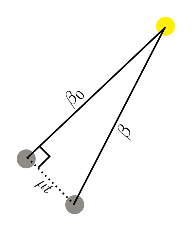
\includegraphics[width=0.2\textwidth]{A_1_12.eps}
\label{fig:12_1}
\caption{An illustration of the motion of lens (gray) across the source (yellow). The initial angle is $\beta_0$, the velocity $\mu$ and final angle is $\beta$.}
\label{fig:amp}
\end{center}
\end{figure}
We are asked to find the net amplification obtained for the two images formed by gravitational lensing. There are a couple of important things here:
\begin{itemize}
\item The lens has a proper motion of $\mu$ milliarcsec per year, and is at the closest approach to the source at $t=0$. Thus, it must mean at the closest approach the velocity and the angular separation between the source and the lens must be perpendicular --  for if there is a component of velocity along the angular separation vector $\beta_0$, there would exist (or would have existed) some other value of closest approach due to the radial motion. This is shown in Fig.~\ref{fig:amp}
\item The initial separation $\beta_0<<\theta_E$, as given in the problem.
\item Any small further motion can be approximated using the Pythagoras theorem.
\end{itemize}
With this information, we can derive the amplification for  our case. Using the same notation as that used in the class, we have the measured angle $\theta$ as:
\begin{equation}
\theta = \frac{1}{2} \{\beta \pm \sqrt{\beta^2+4\theta_E^2}\}
\label{eqn12:1}
\end{equation}
The amplification is given by 
\begin{equation}
A = \frac{\theta d\theta }{\beta d\beta}
\label{eqn12:2}
\end{equation}
Thus, finding out this relation and adding them up for both of the images gives us:
\begin{equation}
\begin{split}
\frac{d\theta}{d\beta} &= \frac{1}{2} \{1\pm\frac{\beta}{\sqrt{\beta^2+4\theta_E^2}}\} \\
\Rightarrow A_{\pm} &= \frac{1}{\beta} \{2\beta \pm \frac{\beta^2}{\sqrt{\beta^2+4\theta_E^2}} \pm \sqrt{\beta^2+4\theta_E^2}\}
\end{split}
\end{equation}
Considering the total magnification as $A = |A_+|+|A_-|$, the $\pm$ terms get added up, and we get:
\begin{equation}
A = \frac{1}{\beta}\frac{\beta^2+2\theta_E^2}{\sqrt{\beta^2+4\theta_E^2}} 
\end{equation}
Referring to Fig.~\ref{fig:amp}, we can write $\beta^2 = \beta_0^2+ \mu^2 t^2$. Using the fact that $\beta_0<<\theta_E$, we get:
\begin{equation}
\begin{split}
A &\approx \frac{1}{\sqrt{\beta_0^2+(\mu t)^2}}\frac{2\theta_E^2}{2\theta_E} \\
\Rightarrow A &\approx \frac{\theta_E/\beta_0}{\sqrt{1+(\mu t/\beta_0)^2}}
\end{split}
\end{equation}
%---------------------------------
\section{Question : 13}
If we consider a star with recombination rate exactly balanced by the ionization rate, we get:
\begin{equation}
\frac{4}{3}\pi r^3 \alpha n^2 = N
\label{eqn13:1}
\end{equation}
where $\alpha$ is the recombination rate density, $r$ is radius of the sphere, $n$ is the number density of the ionized gas, and $N$ is the total rate of ionizing photons. We are given:
\begin{itemize}
\item N = $10^{48}$ photons $sec^{-1}$
\item n = 1 $cm^{-3}$
\item $\alpha$ = $2.59\times 10^{-13}$ $cm^{3}$ $s^{-1}$
\end{itemize}
Calculating r in Eq.~\ref{eqn13:1}, we get:
\begin{center}
$r = 9.7\times 10^{19}$ cm $\approx 10^9 R_\odot$
\end{center}
This is the Stroemgren radius of the region. Now, if 2/3 rd of the recombinations result in Ly$\alpha$, we get the luminosity (with wavelength as 1215 \AA) as:
\begin{equation}
\begin{split}
L_{\alpha} &= \frac{2}{3}N\frac{hc}{\lambda} \\
&=\frac{2}{3}10^{48}\frac{6.6\times10^{-34}\times3\times10^8}{1215\times10^{-10}}\\
&=1.08\times 10^{30}
\end{split}
\end{equation}
Here, we use the fact that recombination rate is equal to the ionization rate. Thus, we get $L_\alpha$ as $10^{30}$ Joule per sec. 
%----------------------------------
\section{Question : 14}
For estimating the fraction of neutral hydrogen in the gas, we are given:
\begin{itemize}
\item n = 10 $cm^{-3}$
\item T = $10^3$ K
\end{itemize}
We know for a hydrogen gas:
\begin{equation}
\frac{x^2}{1-x} = \frac{1}{n}\left(\frac{2\pi m_e kT}{h^2}\right)^{3/2}exp\{-\frac{\phi}{kT}\}
\end{equation}
where, the constants are all obvious, and we take $\phi$ as the ionization potential of hydrogen. Putting the appropriate values and approximating $1-x$ as $x$, we obtain:
$$
x \approx 1.5\times 10^{-24}
$$
However, this is the fraction of ionized Hydrogen. The fraction of neutral hydrogen would be:
$$
1-x \approx 1-5\times 10^{-24} \approx 1
$$
So there is a very small amount of ionization, but it is not much. 
\section{Question : 15}
We are given two objects -- one, a QSO at a redshift of 3, and a H1 cloud at a redshift of 2. We are also given the intrinsic spectrum of the QSO, and the Hydrogen ionizing cross section. These are:
\begin{itemize}
\item Intrinsic luminosity $L_\lambda =  10^{43}\left(\frac{\lambda}{3000}\right)^{-1}$
\item $\sigma(\lambda) = 6.8\times 10^{-18}\left(\frac{\lambda}{\lambda_0}\right)^3$, where $\lambda_0 = 912$\AA, only from $\lambda \leq \lambda_0$
\item Column density $N = 7\times10^{16}$ $cm^{-2}$
\end{itemize}
As the light travels from the QSO to us, the following events will happen:
\begin{enumerate}
\item Red-shifted at the H1 cloud.
\item Thomson and Bound-free scattering at the cloud.
\item Ly $\alpha$ break at 921 {\AA} locally.
\item Red-shifted from cloud to us.
\item There is also the reduction of flux due to distance, which goes as inverse square. 
\end{enumerate}
The optical depth for the two cases would be:
$$ \tau_T = 4.2\times 10^{-8}$$
$$ \tau(\lambda) = 0.476 \left(\frac{\lambda_0}{\lambda}\right)^3$$
Now, for the calculation of distance, an online calculator was used~\cite{Calc}. The default values were used for finding the parameters:
\begin{center}
\begin{tabular}{c|c}
\hline 
$H_0$ & 69.6 \\
$\Omega_M$ & 0.286 \\
$\Omega_{vac}$ & 0.714 \\
\hline
\end{tabular}
\end{center}
These values result in a distance measure of $84.855$ GLy between the QSO and us, and $51.59$ GLy between the H1 cloud and us. This is used for flux calculation here. 

The spectrum is constructed as follows:
\begin{enumerate}
\item Define a range of wavelengths at Earth.
\item Use $\lambda' \rightarrow \lambda/(1+z)$ to obtain the relevant ranges at QSO and H1 cloud.
\item Find $L_{\lambda',qso}$, and the decay factor at the cloud.
\item Redshift the two to Earth, and reduce them by $r^2$ 
\item Multiply the spectra.
\end{enumerate}
The spectra are shown in Fig.~\ref{fig:qso_mult}.
\begin{figure}[!htpb]
\centering
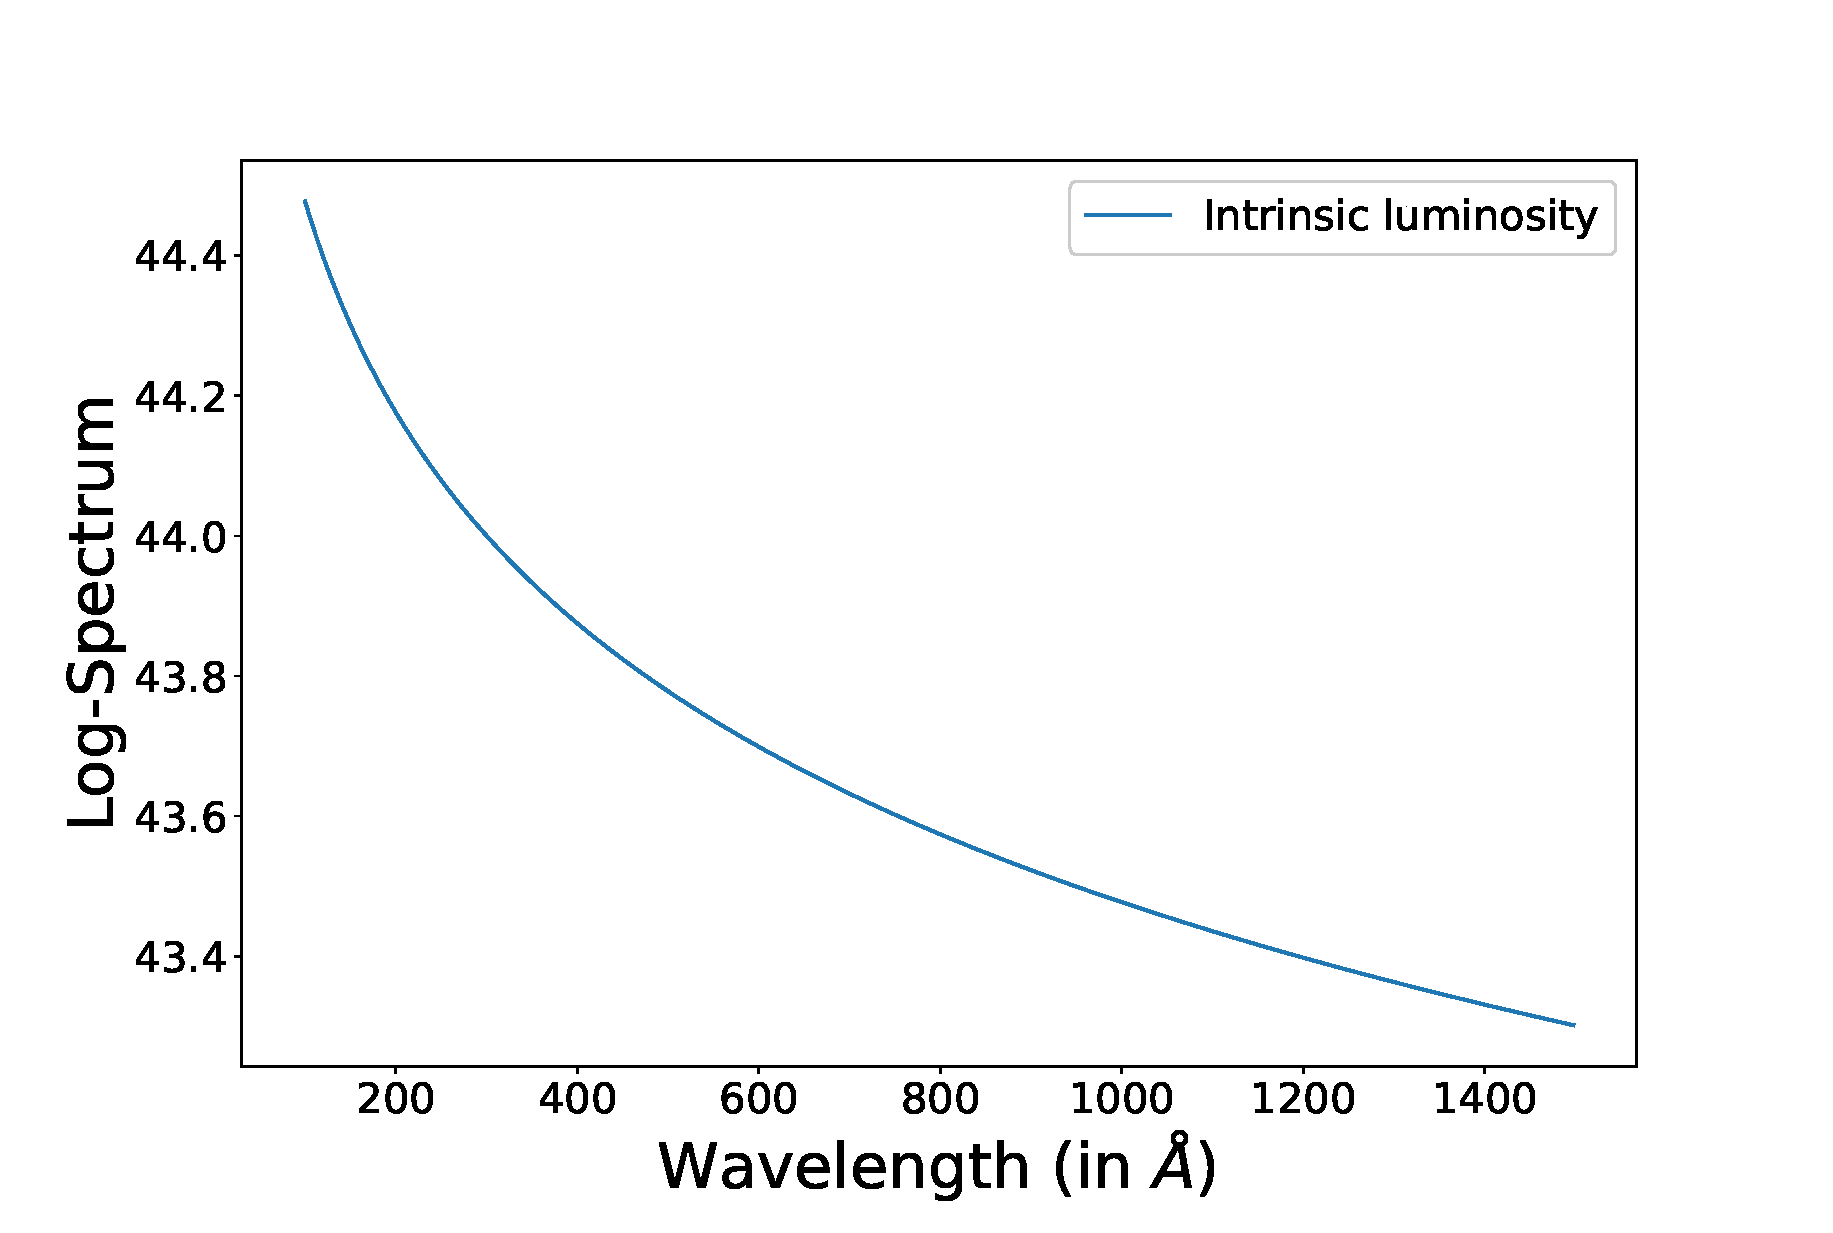
\includegraphics[width=0.4\linewidth]{Intrinsic.eps}
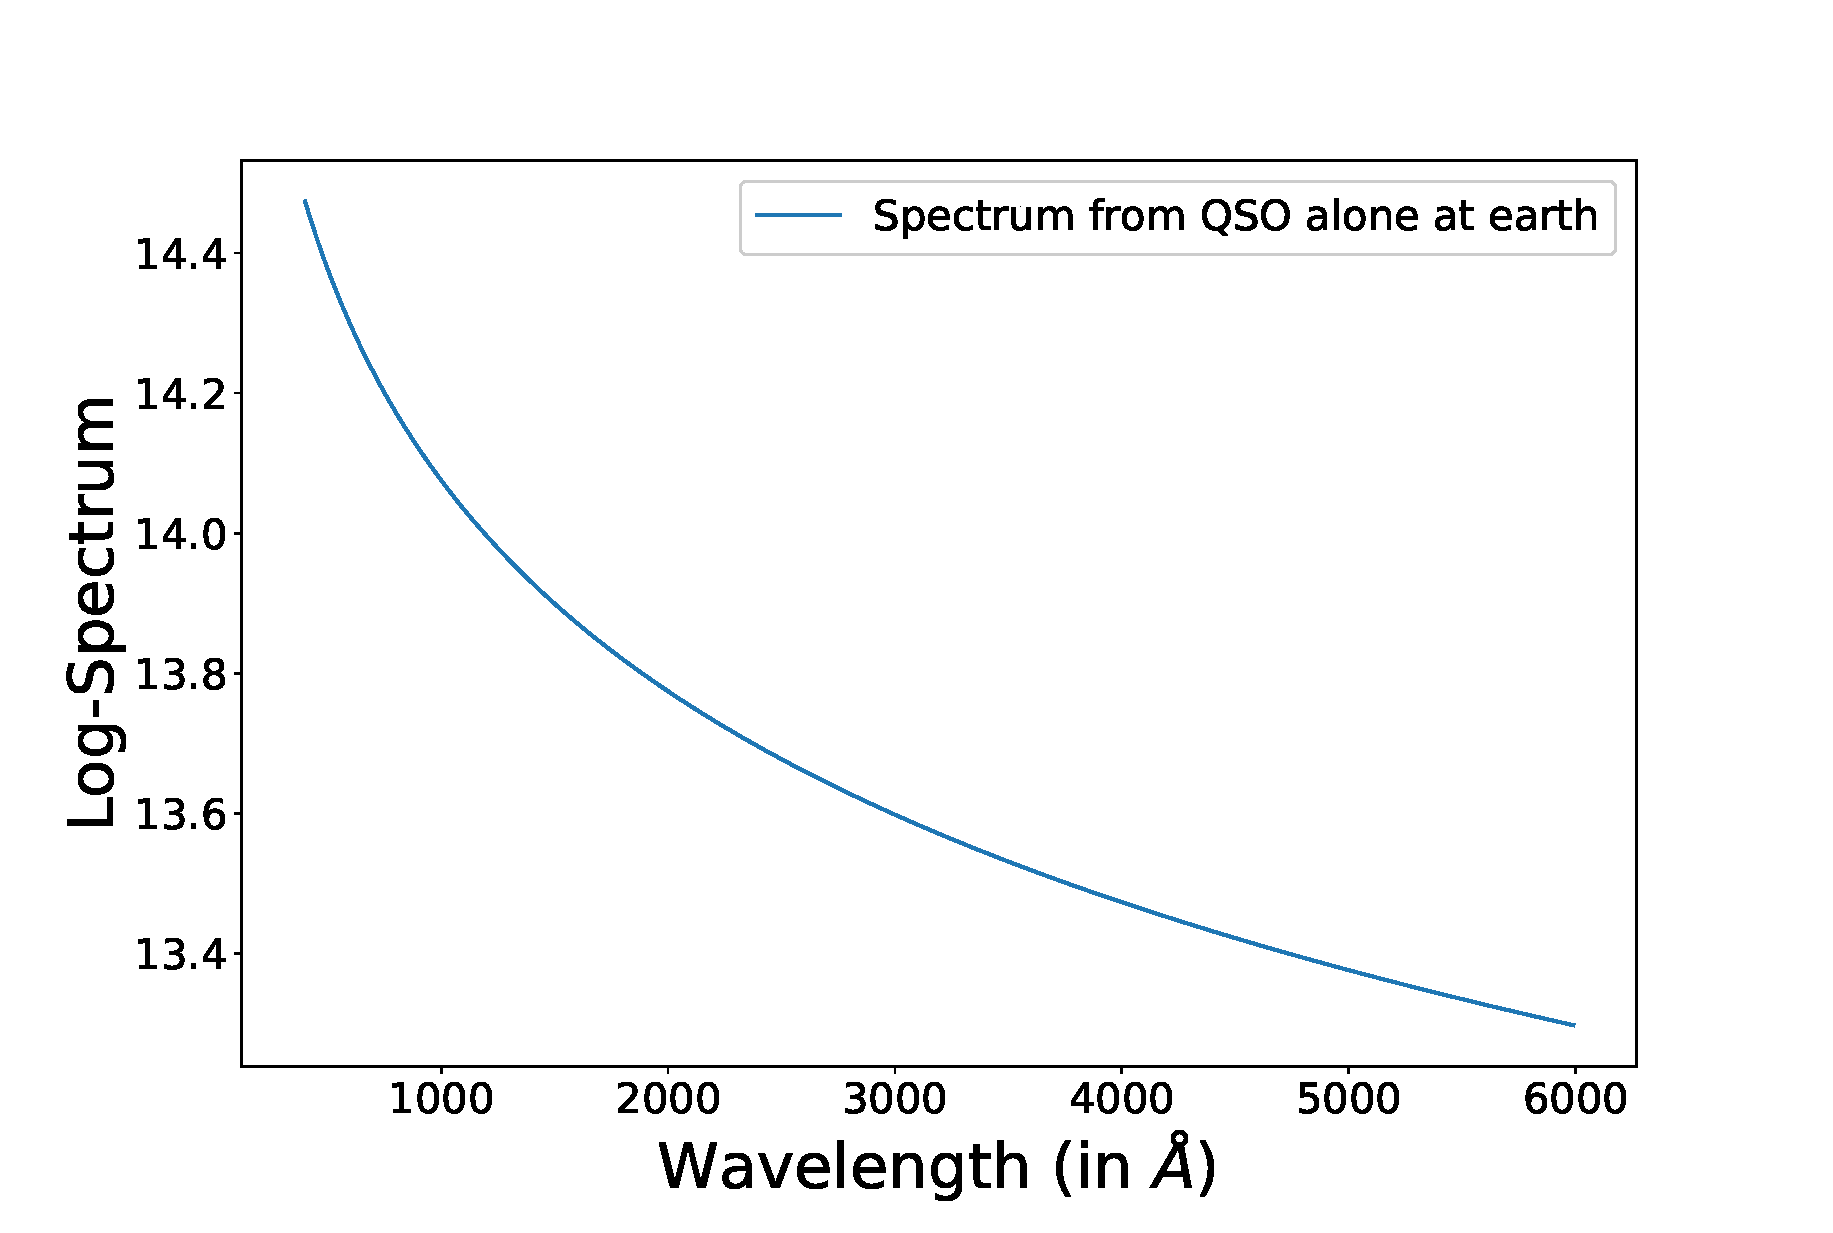
\includegraphics[width=0.4\linewidth]{QSO_Earth.eps}
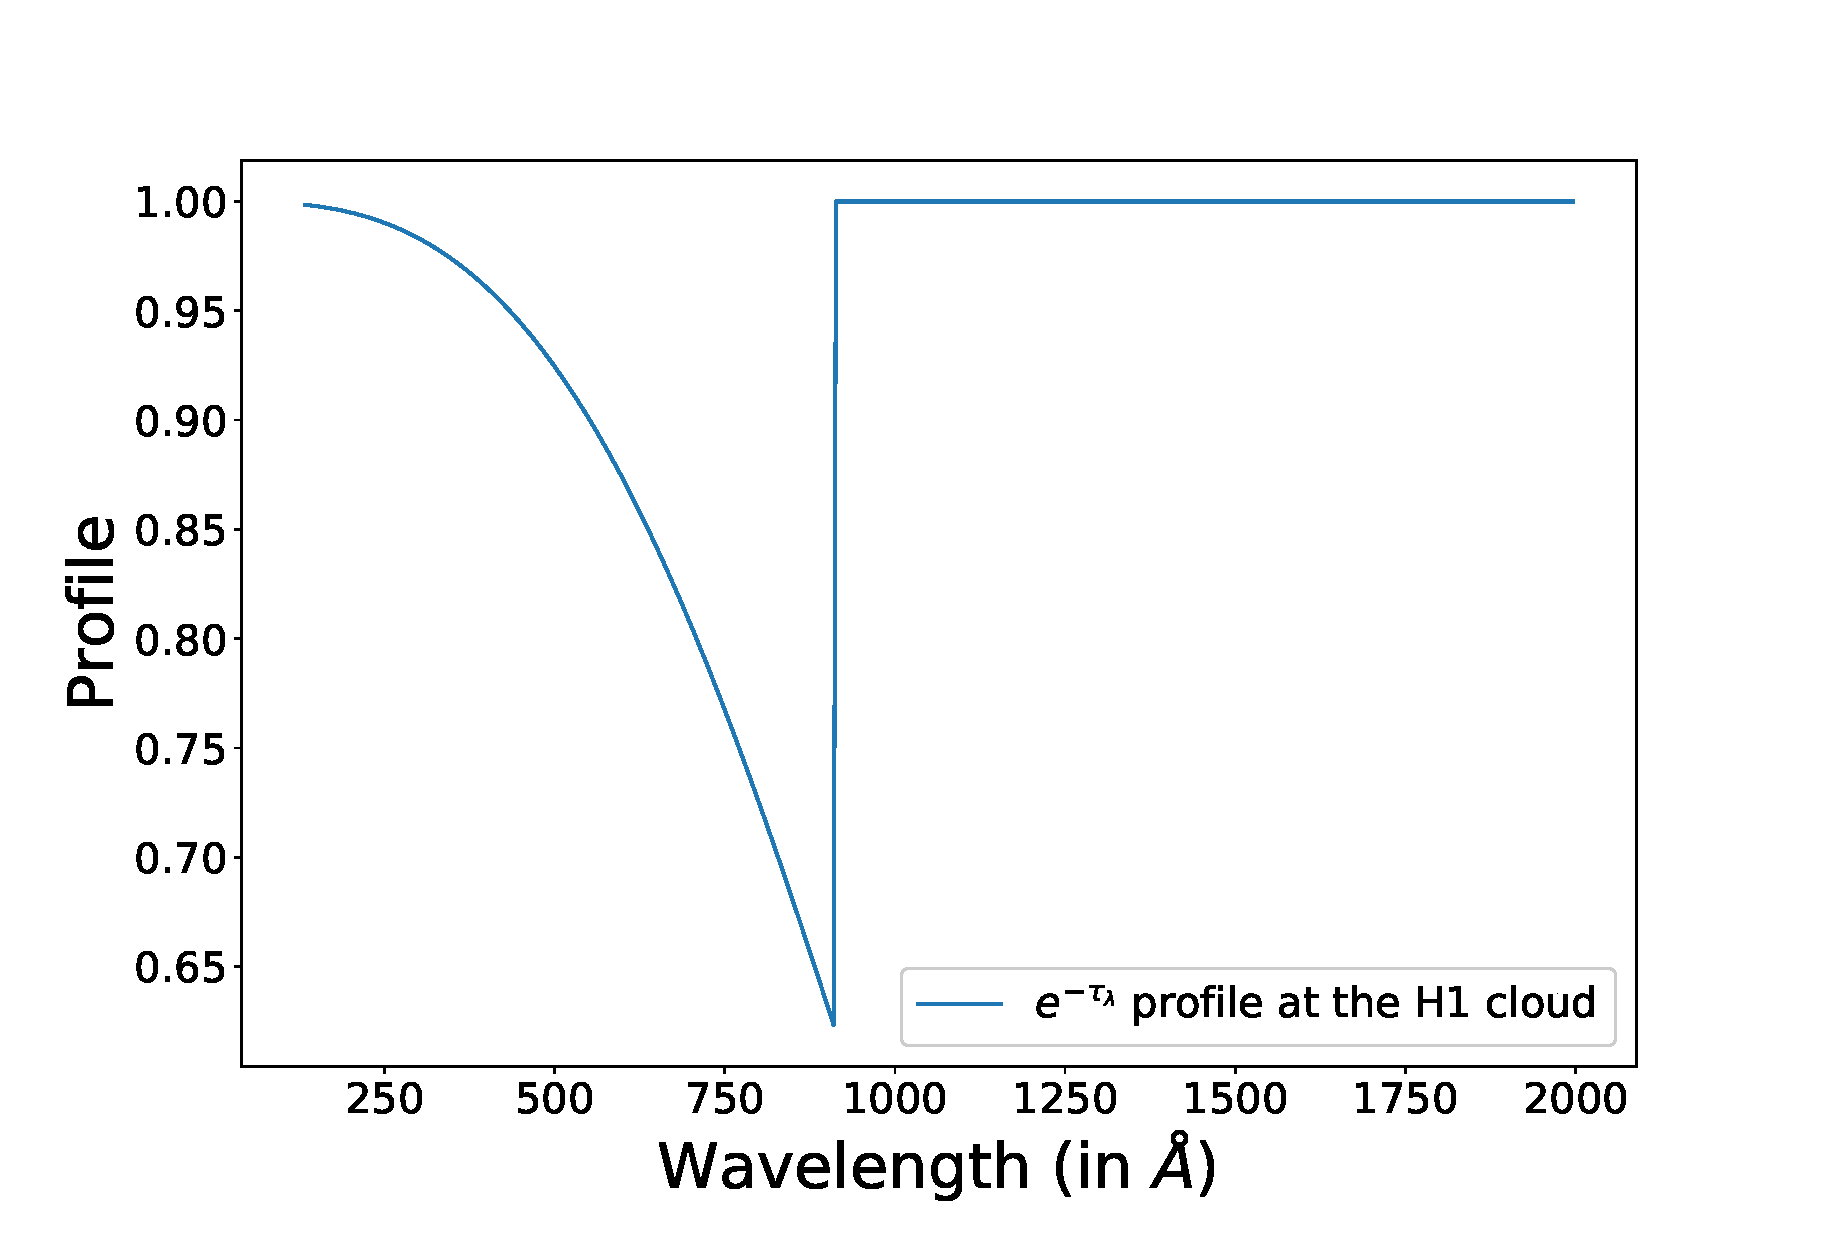
\includegraphics[width=0.4\linewidth]{H1_Earth.eps}
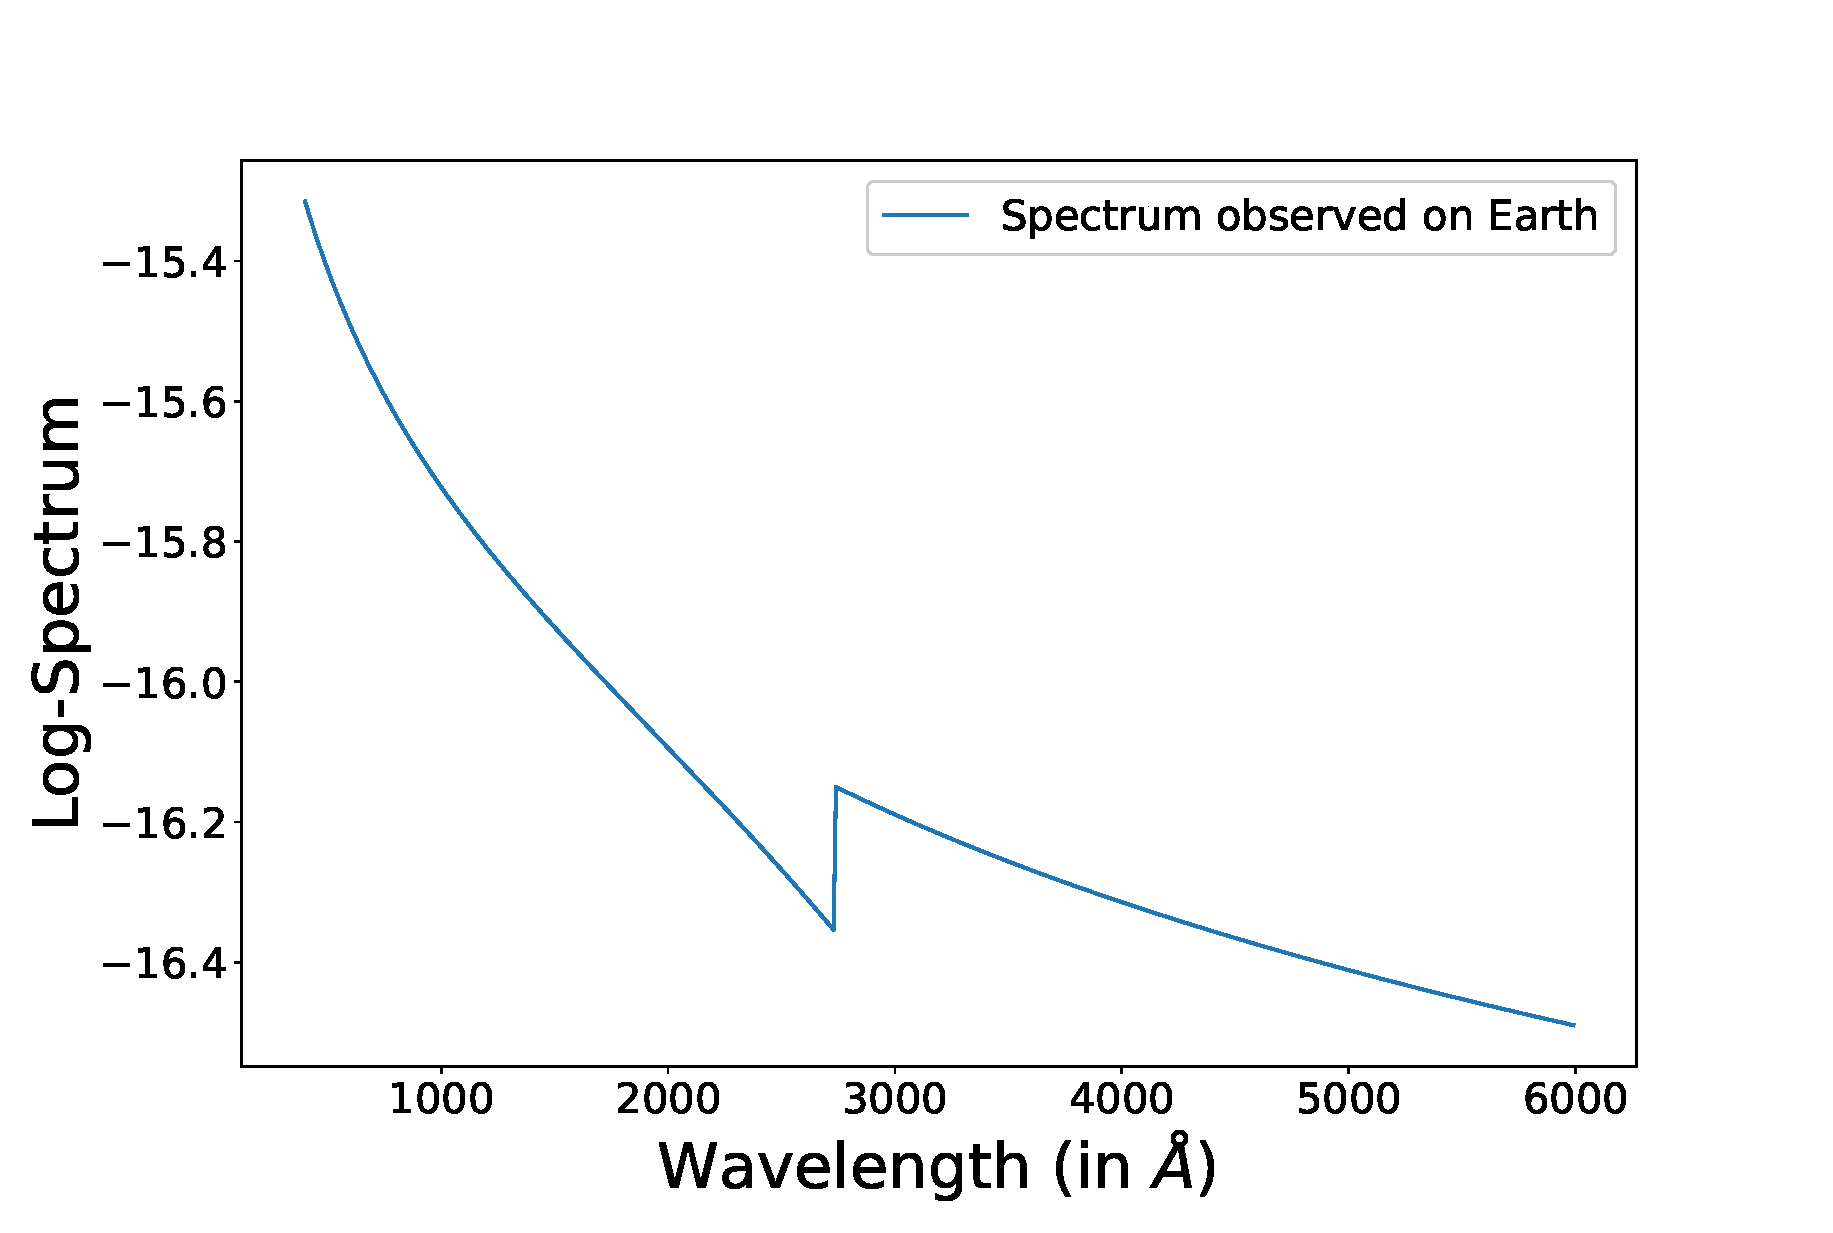
\includegraphics[width=0.4\linewidth]{Earth.eps}
\caption{From top left clockwise: Intrinsic luminosity spectrum of the QSO; Spectrum of flux obtained at Earth if there were no cloud between the QSO and us; Spectrum of flux as obtained on Earth; Absorption profile $e^{-\tau_{\lambda}}$(or rather, transmission profile) of the H1 cloud.}
\label{fig:qso_mult}
\end{figure}%

\bibliographystyle{unsrt}
\bibliography{refs}
\end{document}
